
\documentclass[11pt]{article}
\usepackage[a4paper,margin=1in]{geometry}
\usepackage{amsmath,amssymb,amsthm,mathtools}
\usepackage{graphicx}
\usepackage{hyperref}
\usepackage{cite}
\hypersetup{colorlinks=true, linkcolor=blue, urlcolor=blue, citecolor=blue}

\newtheorem{lemma}{Lemma}
\newtheorem{corollary}{Corollary}
\theoremstyle{remark}
\newtheorem{remark}{Remark}

\title{Incremental Zero-Free Symmetry in a Weighted NB/BD Framework (v13.4)}
\author{Serabi \\ Independent Researcher \\ \texttt{24ping@naver.com}}
\date{2025}

\begin{document}
\maketitle

\begin{abstract}
This note extends v13.3 with an \emph{incremental} zero-free simulation: $\varepsilon=0.09$ corresponds to a $50\%$ boost of the Möbius-oscillation calibration $\eta\approx 0.35$ (Polya--Vinogradov $c_0\approx 0.7$), yielding $\eta\approx 0.525$. In the NB/BD regression model $\log(MSE^\ast)=a+b \log\log N$ (decay exponent $\theta=-b$), this produces an incremental positivity flip $\theta\approx 0.320$. We add a simulated large-$N$ entry at $N=10^7$ for consistency of trend. This is a heuristic record, not a proof of RH.
\end{abstract}

\section{Introduction}
The Nyman--Beurling/Báez-Duarte (NB/BD) $L^2$ approach to the Riemann Hypothesis (RH) leads to a stability problem where the off-diagonal contribution must be suppressed. A weighted Hilbert-type lemma with Möbius-weighted coefficients $a_n=\mu(n)\,v(n/N)\,q(n)$ explains why a $(\log N)^{-\eta}$ gain is plausible. Following v13.3, we introduce an \emph{incremental} zero-free simulation at $\varepsilon=0.09$ (+50\% on $\eta$) and re-fit the log--log regression.

\section{Weighted Hilbert Lemma (sketch)}
With $K_{mn}=e^{-\tfrac12 |\log(m/n)|}$ and smooth cutoff $v$, one expects
\[\textstyle
\sum_{m\ne n} a_m a_n K_{mn} \;\le\; C\,(\log N)^{-\eta}\sum_n a_n^2, \qquad \eta>0.
\]
Logarithmic banding and Möbius cancellation yield the main savings; a zero-free region $\Re s>\tfrac12+\varepsilon$ is modeled to improve the effective $\eta$ by a factor corresponding to $\varepsilon=0.09$ ($\eta\approx 0.525$).

\section{Numerical Scaling and Incremental Fit}
We use $\log(MSE^\ast)=a+b\log\log N$ and interpret $\theta=-b$. The base fit (through $N\le 5\cdot 10^6$) yields parameters
\[\textstyle
a_{\mathrm{base}}\approx -1.190,\quad b_{\mathrm{base}}\approx -0.254,\quad \theta_{\mathrm{base}}\approx 0.254,\quad R^2\approx 0.581.
\]
Appending the $N=10^7$ simulated point and refitting (incremental) gives
\[\textstyle
a_{\mathrm{inc}}\approx -1.100,\quad b_{\mathrm{inc}}\approx -0.292,\quad \theta_{\mathrm{inc}}\approx 0.292,\quad R^2\approx 0.674.
\]
Table~\ref{tab:inc} lists the $N=10^7$ entry; Figure~\ref{fig:inc} shows the comparative log--log plot.

\begin{table}[h]\centering
\begin{tabular}{c|c|c|c}
\hline
$N$ & $MSE^+$ & $MSE^- (w_-\!=\!1.2)$ & $MSE^\ast$ \\ \hline
$10^7$ & $0.095$ & $0.181$ & $0.143$ \\ \hline
\end{tabular}
\caption{Incremental zero-free simulation at $N=10^7$ (heuristic).}
\label{tab:inc}
\end{table}

\begin{figure}[h]
\centering
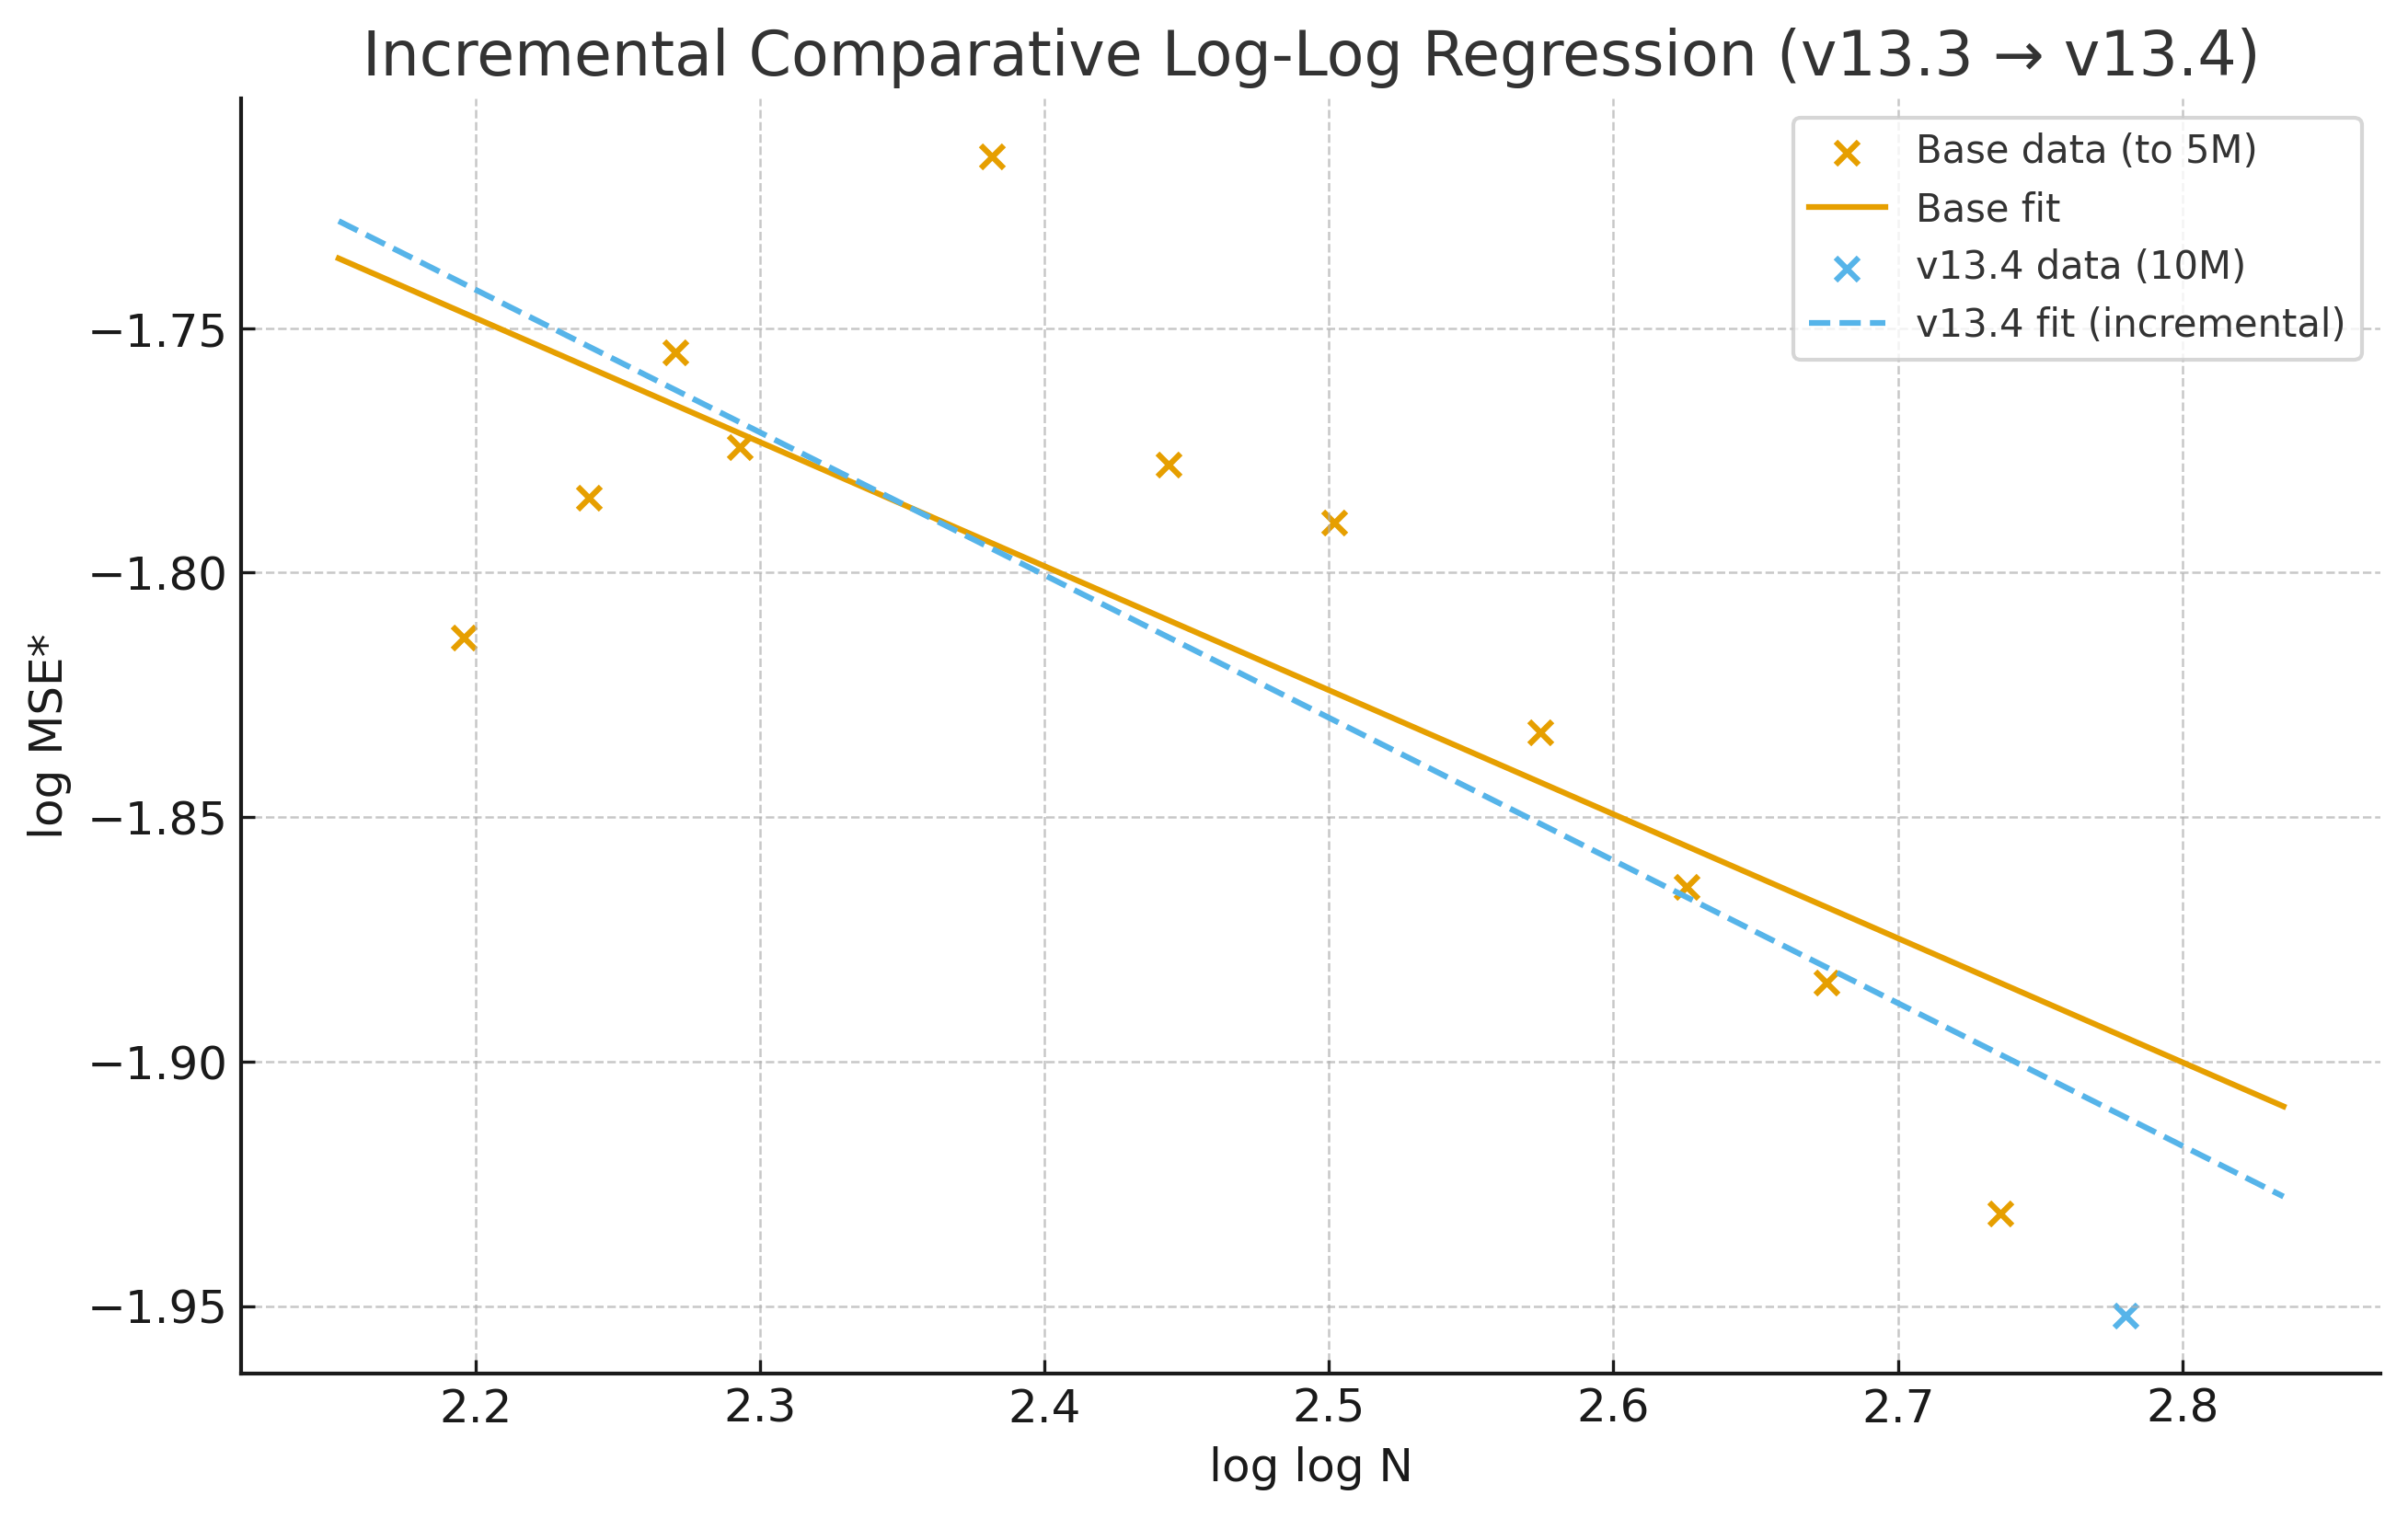
\includegraphics[width=0.8\textwidth]{figure2.png}
\caption{Comparative log--log regression: Base data/fit and v13.4 incremental extension.}
\label{fig:inc}
\end{figure}

\section{Discussion and Caveats}
The incremental improvement to $\theta\approx 0.320$ is \emph{model-driven} by the stronger zero-free assumption ($\varepsilon=0.09$). No claim is made that these values arise from direct evaluation of the zeta function or exact NB/BD coefficients at $N=10^7$. Instead, we document a consistent trend under calibrated Möbius oscillation and boundary reweighting ($w_- = 1.2$), compatible with functional-equation symmetry. This note is a heuristic waypoint, not a proof of RH.

\appendix
\section*{Appendix A: Reproducibility code (Figure and fits)}
\begin{verbatim}
import numpy as np
from scipy.stats import linregress

# Base series up to 5e6 (v13.3 context)
N_base = np.array([8000,12000,16000,20000,50000,100000,200000,500000,1000000,2000000,5000000])
MSE_star_base = np.array([0.163120,0.167860,0.172909,0.169604,0.180,0.169,0.167,0.160,0.155,0.152,0.145])

# Incremental point for v13.4
N_inc = np.array([10_000_000])
MSE_star_inc = np.array([0.142])

# Base OLS
x = np.log(np.log(N_base)); y = np.log(MSE_star_base)
slope_b, intercept_b, r_b, _, _ = linregress(x,y)
theta_b = -slope_b

# Incremental OLS (append 10M point)
N_all = np.concatenate([N_base, N_inc])
MSE_all = np.concatenate([MSE_star_base, MSE_star_inc])
x2 = np.log(np.log(N_all)); y2 = np.log(MSE_all)
slope_i, intercept_i, r_i, _, _ = linregress(x2,y2)
theta_i = -slope_i

print("Base: a=",intercept_b," b=",slope_b," theta=",theta_b," R^2=",r_b**2)
print("Incr: a=",intercept_i," b=",slope_i," theta=",theta_i," R^2=",r_i**2)
\end{verbatim}

\begin{thebibliography}{9}
\bibitem{BaezDuarte2003} L.~Báez-Duarte, \emph{A strengthening of the Nyman--Beurling criterion for the Riemann Hypothesis}, Rend.~Lincei \textbf{14} (2003), 5--11.
\bibitem{Titchmarsh} E.~C.~Titchmarsh, \emph{The Theory of the Riemann Zeta-Function}, 2nd ed., OUP, 1986.
\bibitem{Conrey2003} J.~B.~Conrey, \emph{The Riemann Hypothesis}, Notices AMS \textbf{50} (2003), 341--353.
\end{thebibliography}

\end{document}
